% !TEX program = xelatex
\documentclass{article}
\usepackage{/Users/Jay/LaTeX/cs}
\usepackage{/Users/Jay/LaTeX/matlab}
\usepackage{/Users/Jay/LaTeX/xeCJK}

\newcommand{\hmwkClass}{Digital Image Processing, Spring 2018}
\newcommand{\hmwkTitle}{Proposal Report}
\newcommand{\hmwkDueDate}{May 15, 2018}
\newcommand{\tb}{\textbf}

\begin{document}

\thispagestyle{empty}
\section*{\hmwkClass \\
    \normalsize{\hmwkTitle} \\
    \normalsize{DUE DATE: \hmwkDueDate}
}

\hfill{Team 10: \, R06945003 \, 林鈺盛 \, B03902129 \, 陳鵬宇} \\

\section*{Paper title}

Title: Fast Image Processing with Fully-Convolutional Networks \\
Conference: ICCV 2017 \\
Authors: Qifeng Chen, Jai Xu Intel Labs and Vladlen Koltun

\section*{Motivation}

Image processing can be used in everywhere. Like robotic navigation systems, traffic, healthcare, camera edge technology, etc. Faster image processing can save us tons of time. Learning how to accelerate the procedure of image processing is undoubtedly worthy.

\section*{Problem definition}

Use convolution neural network (CNN) to implement image processing methods mentioned in class.

\section*{Algorithm}

\subsubsection*{Preliminaries}

Given:

\begin{itemize}
    \item \tb I: image in RGB space and
    \item $f$: operator, where \tb{I} and $f(\tb I)$ have the same resolution.
\end{itemize}

Our goal is:

\begin{itemize}
    \item to approximate $f$ with another operator $\hat f$, that is $f(\tb I) \approx \hat f(\tb I)$ for all images and
    \item to find a broadly applicable image processing operator.
\end{itemize}

There are three desirable criteria we want to meet with:

\begin{enumerate}
    \item Accuracy
    \item Speed
    \item Compactness
\end{enumerate}

\subsubsection*{Context Aggregation Networks (CAN)}

The primary architecture the paper used is \tb{multi-scale context aggregation network (CAN)}

Now let's describe the parameterization in detail.

The data lay out over layers: $\{\tb L^0, \dots, \tb L^d\}$.

\begin{itemize}
    \item Dimension of $\tb L^0$ (input) and $\tb L^d$ (output): $m \times n \times 3$.
    \item Dimension of $\tb L^s$ ($1 \le s \le d - 1$): $m \times n \times w$, where $w$ is the width (features) of each layer.
\end{itemize}

$\tb L^s$ can be computed from the previous layer $\tb L^{s - 1}$ as follows:

$$\tb L_i^s = \Phi\bigg( \Psi^s \bigg(b_i^s + \sum\limits_j \tb L_j^{s - 1} *_{r_s} \tb K_{i, j}^s \bigg)\bigg)$$

and $\Psi^s(x)$ is computed as follow:

$$\Psi^s(x) = \lambda_s x + \mu_s BN(x),$$

where $\lambda_s, \mu_s \in \mathbb R$ are learned scalar weights and $BN$ is the batch normalization operator. We'll keep training these two scalars for each iteration.

Specically, for image coordinates $x$:

$$(\textbf L_j^{s - 1} *_{r_s} \textbf K_{i,j}^s) (x) = \sum\limits_{a + r_s b = x} \textbf L_j^{s - 1}(a) \textbf K_{i,j}^s(b)$$

Perform dilated convolution needs to specify the kernel size, it looks like: \\

\begin{center}
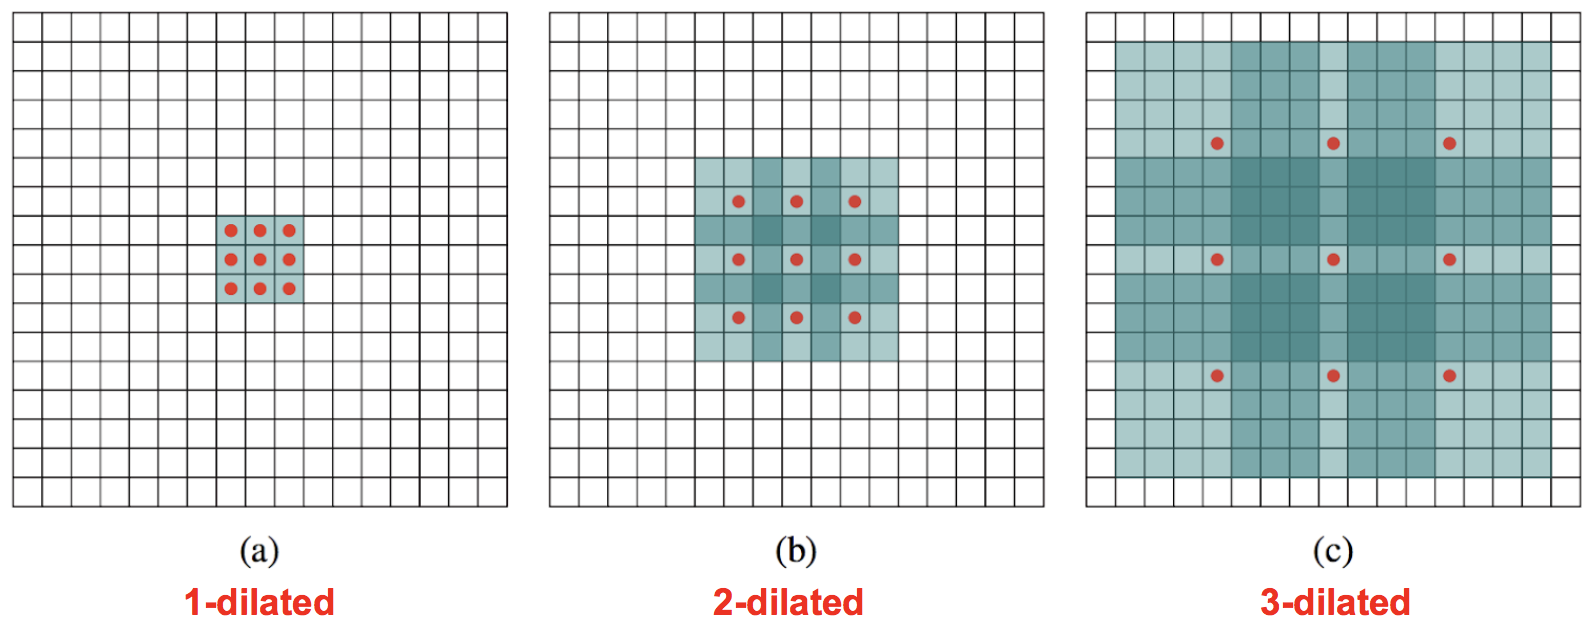
\includegraphics[width=0.8\textwidth]{img/dilated.png}
\end{center}

\subsubsection*{Training}

The network is trained on a set of input-output pairs that contain images before and after the application of original operator: $\mathcal D = \{\tb I_i, f(\tb I_i)\}$.

\begin{itemize}
    \item the parameters of the network are the kernel weights $\mathcal K = \{\tb K_{i, j}^s\}_{s, i, j}$ and
    \item the scalar biases $\mathcal B = \{b_i^s\}_{s, i}$.
\end{itemize}

Therse parameters are optimized to fit the action of the operator $f$ across all images in the training set.

We train with an image-space regression loss:

$$\ell(\mathcal K, \mathcal B) = \sum\limits_i \frac{1}{N_i} ||\hat f(\tb I_i; \mathcal K, \mathcal B) - f(\tb I_i)||^2,$$

where $N_i$ is the number of pixels in image $\tb I_i$.

\section*{Extensions}

\subsubsection*{Parameterized operators}

Image processing operator can have parameters that control its action.

\begin{itemize}
    \item image smoothing operator:$\lambda$
    \item higher $\lambda$ leads to more aggressive smoothing
\end{itemize}

Therefore, we can add an input channel that is used to communicate the parameter's value to the network.

\subsubsection*{Single network}

\begin{itemize}
    \item Augment the input layer by adding 10 additional channels, where each channel is a binary indicator that corresponds to one of the 10 operators.
    \item Remarkably, a single compact network that represents all $10$ operators achieves high accuracy.
\end{itemize}

\section*{Expected results}

Use CNN model to implement \textsl{\tb{edge detection, half toning, noise removal}}, etc.

Here is the result of the paper: \\

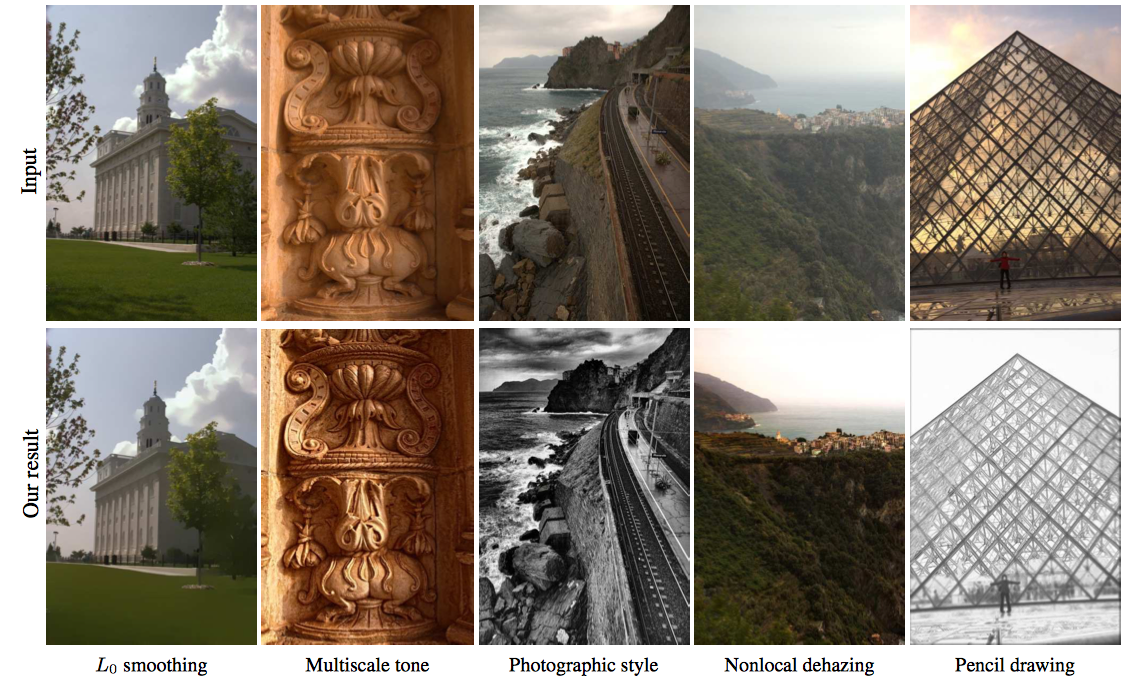
\includegraphics[width=\textwidth]{img/img.png}

\section*{Reference}

[1] \href{http://openaccess.thecvf.com/content_ICCV_2017/papers/Chen_Fast_Image_Processing_ICCV_2017_paper.pdf}{Fast Image Processing with Fully-Convolutional Networks}

[2] \href{https://arxiv.org/pdf/1511.07122.pdf}{Multi-scale context aggregation by dilated convolutions}

\end{document}